\section{Algorithm Specification}

\subsection*{\textit{Version 1.0}}

\subsection{Introduction}

The CIShell Platform has been specifically designed around the idea of the
algorithm. It is the central and most important concept. Algorithms are fully
defined and self-contained bits of execution. They can do many things from data
conversion, data analysis, and can even spawn whole outside programs if it needs
to. Algorithms are very well defined black boxes in that what can come into and
out of the algorithm is specified in each algorithm's metadata. Other than that,
CIShell makes no attempt to understand the algorithm.

To be recognized by CIShell, an \class{AlgorithmFactory} must be registered with
OSGi's Service Registry. The service registry requires three things when
registering: An interface (\class{AlgorithmFactory}), an implementation, and a
\class{Dictionary} of metadata. The algorithm developer provides the
implementation and metadata. The metadata helps to differentiate and define the
algorithm for search and discovery, see section \ref{algMetaData}.

An algorithm defines its inputs in two ways. First, the input data is defined in
the algorithm's service metadata. Second, the acceptable user-entered parameters
are defined in a \class{MetaTypeProvider}, see section \ref{GUISpec}.

Figure \ref{fig:algExecWorkflow} shows the typical flow of information into and
out of an algorithm. First the input parameter specification is pulled from the
\class{AlgorithmFactory}. If parameters are needed, then a UI is created and user
inputs are entered. To create an \class{Algorithm}, the \class{AlgorithmFactory}
is passed the user-entered parameters, zero or more pieces of data, and a
\class{CIShellContext}. The \class{Algorithm} is then executed and produces zero
or more pieces of data.

\begin{figure}[htb!]
\centering
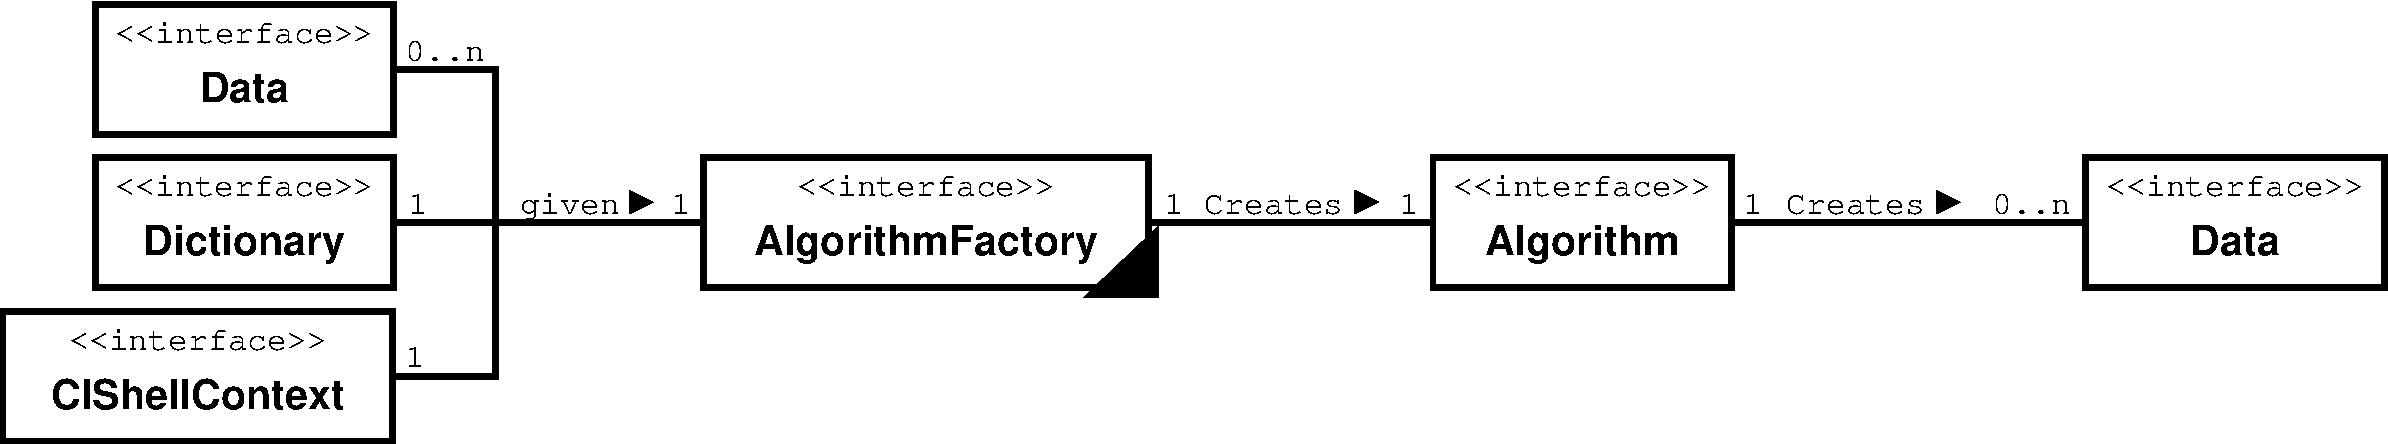
\includegraphics[width=150mm]{../img/algExecWorkflow.pdf}
\caption{Algorithm Execution Workflow}
\label{fig:algExecWorkflow}
\end{figure}

\subsection{Optional Interfaces}

Algorithm developers may augment algorithms with additional interfaces to enhance
parts of the execution workflow. An \class{AlgorithmFactory} can also implement
the \class{DataValidator} interface to validate the data beyond the data format
validation that an application should provide ahead of time. An \class{Algorithm}
can implement \class{ProgressTrackable} to allow for more detailed monitoring and
control of an \class{Algorithm}'s progress while executing. See each interface's
documentation for more details.

\subsection{Algorithm Service Metadata}
\label{algMetaData}

When an algorithm is registered with OSGi's service registry, a dictionary of
metadata is provided. Since the algorithm itself is a black box, the metadata is
used to provide information about the algorithm. Information such as the format
of each \class{Data} item to be inputted and outputted is provided. In addition to the
mechanics of the algorithms, interesting data such as the authors, label, urls,
and description are provided. This metadata can be searched by anyone using
OSGi's service registry to find relevant algorithms for use.

\comments{Lots more to do here. Need to define what is/isn't mandatory for each
algorithm type. Perhaps some figures\ldots}


